%%%%%%%%%%%%%%%%%%%%%%%%%%%%%%%%%%%%%%%%%%%%%%%%%%%%%%%%%%%%%%%%%%%%%%%%%%%%%%%%%%%%%%
% author                : louis tomczyk
% date of production    : 2024-03-03
% licence               : cc-by-nc-sa
%                         Attribution - Non-Commercial - Share Alike 4.0 International
%%%%%%%%%%%%%%%%%%%%%%%%%%%%%%%%%%%%%%%%%%%%%%%%%%%%%%%%%%%%%%%%%%%%%%%%%%%%%%%%%%%%%%

\bfig
	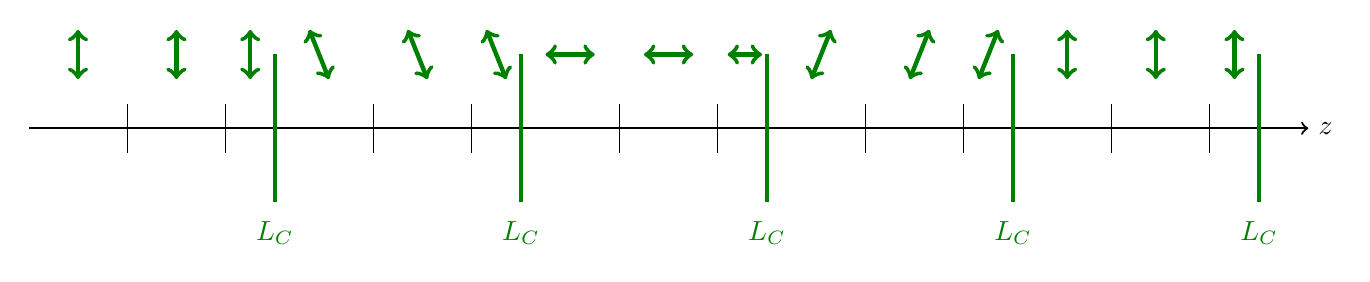
\begin{tikzpicture}[scale = 1.25]
		\draw[thick, ->] (0,0) --++ (13,0)node[right]{$z$};
		\foreach \z in {1,2,3.5,4.5,6,7,8.5,9.5,11,12}
		{
        \draw (\z,-0.25)node[below = 3pt]{$\Lbp$}--++ (0,0.5);
		}
    		\foreach \z in {2.5,5,7.5,10,12.5}
		{
			\draw[ultra thick, green!50!black] (\z,-0.75)node[below = 3pt]{$L_C$} --++ (0,1.5);
		}
		\draw[<->,ultra thick, green!50!black] (0.5,1)--++ (0,-0.5);
		\draw[<->,ultra thick, green!50!black] (1.5,1)--++ (0,-0.5);
		\draw[<->,ultra thick, green!50!black] (2.25,1)--++ (0,-0.5);

		\draw[<->,ultra thick, green!50!black] (2.85,1)--++ (0.2,-0.5);
		\draw[<->,ultra thick, green!50!black] (3.85,1)--++ (0.2,-0.5);
		\draw[<->,ultra thick, green!50!black] (4.65,1)--++ (0.2,-0.5);

		\draw[<->,ultra thick, green!50!black] (5.25,0.75)--++ (0.5,0);
		\draw[<->,ultra thick, green!50!black] (6.25,0.75)--++ (0.5,0);
		\draw[<->,ultra thick, green!50!black] (7.1,0.75)--++ (0.35,0);

		\draw[<->,ultra thick, green!50!black] (7.95,0.5)--++ (0.2,+0.5);
		\draw[<->,ultra thick, green!50!black] (8.95,0.5)--++ (0.2,+0.5);
		\draw[<->,ultra thick, green!50!black] (9.65,0.5)--++ (0.2,+0.5);

		\draw[<->,ultra thick, green!50!black] (10.55,0.5)--++ (0,+0.5);
		\draw[<->,ultra thick, green!50!black] (11.45,0.5)--++ (0,+0.5);
		\draw[<->,ultra thick, green!50!black] (12.25,0.5)--++ (0,+0.5);

	\end{tikzpicture}
	\caption{Évolution de l'état de polarisation (flèche verte) au cours des
	la propagation dans la fibre quand $L_C>\Lbp$.}
	\label{fig:LC_Lbp}
\efig
